% TikZ code generated by Python script for Common Link Graph visualization
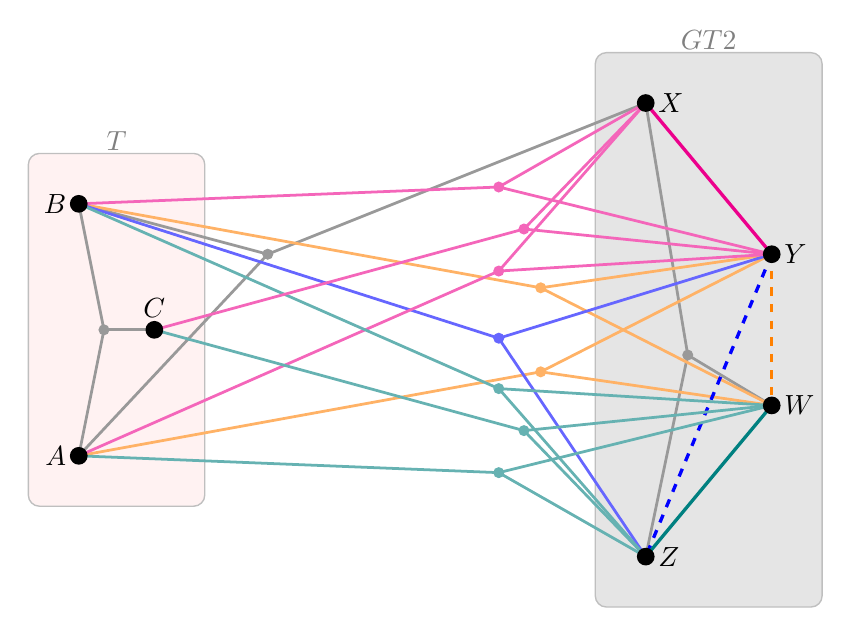
\begin{tikzpicture}[scale=0.8]
% Vertex coordinates
\coordinate (A) at (0.00, 1.60);
\coordinate (B) at (0.00, 5.60);
\coordinate (C) at (1.20, 3.60);
\coordinate (X) at (9.00, 7.20);
\coordinate (Y) at (11.00, 4.80);
\coordinate (Z) at (9.00, 0.00);
\coordinate (W) at (11.00, 2.40);
% Hyperedge root coordinates
\coordinate (R0) at (6.667, 4.533);
\coordinate (R1) at (6.667, 5.867);
\coordinate (R2) at (7.333, 4.267);
\coordinate (R3) at (6.667, 1.333);
\coordinate (R4) at (6.667, 2.667);
\coordinate (R5) at (3.000, 4.800);
\coordinate (R6) at (7.333, 2.933);
\coordinate (R7) at (6.667, 3.467);
\coordinate (R8) at (0.400, 3.600);
\coordinate (R9) at (7.067, 5.200);
\coordinate (R10) at (7.067, 2.000);
\coordinate (R11) at (9.667, 3.200);
% Draw background boxes for T and V \ T
\draw[fill=pink!20, rounded corners, line width=0.5pt, draw=gray!50] (-0.80, 0.80) rectangle (2.00, 6.40);
\node at (0.60, 6.40) [anchor=south, inner sep=1pt, text=gray] {$T$};
\draw[fill=gray!20, rounded corners, line width=0.5pt, draw=gray!50] (8.20, -0.80) rectangle (11.80, 8.00);
\node at (10.00, 8.00) [anchor=south, inner sep=1pt, text=gray] {$\link{G}{T}{2}$};
% Draw hyperedges with |H n T| > k-j (dashed gray, background)
\draw[line width=1.0pt, color=gray!80!white, solid] (R5) -- (A);
\draw[line width=1.0pt, color=gray!80!white, solid] (R5) -- (B);
\draw[line width=1.0pt, color=gray!80!white, solid] (R5) -- (X);
\fill[gray!80!white] (R5) circle (2.5pt);
\draw[line width=1.0pt, color=gray!80!white, solid] (R8) -- (A);
\draw[line width=1.0pt, color=gray!80!white, solid] (R8) -- (B);
\draw[line width=1.0pt, color=gray!80!white, solid] (R8) -- (C);
\fill[gray!80!white] (R8) circle (2.5pt);
\draw[line width=1.0pt, color=gray!80!white, solid] (R11) -- (X);
\draw[line width=1.0pt, color=gray!80!white, solid] (R11) -- (Z);
\draw[line width=1.0pt, color=gray!80!white, solid] (R11) -- (W);
\fill[gray!80!white] (R11) circle (2.5pt);
% Draw hyperedges contributing to 'almost' links (dashed colored)
\draw[line width=1.0pt, color=orange!60!white, solid] (R2) -- (B);
\draw[line width=1.0pt, color=orange!60!white, solid] (R2) -- (Y);
\draw[line width=1.0pt, color=orange!60!white, solid] (R2) -- (W);
\fill[orange!60!white] (R2) circle (2.5pt);
\draw[line width=1.0pt, color=orange!60!white, solid] (R6) -- (A);
\draw[line width=1.0pt, color=orange!60!white, solid] (R6) -- (Y);
\draw[line width=1.0pt, color=orange!60!white, solid] (R6) -- (W);
\fill[orange!60!white] (R6) circle (2.5pt);
\draw[line width=1.0pt, color=blue!60!white, solid] (R7) -- (B);
\draw[line width=1.0pt, color=blue!60!white, solid] (R7) -- (Y);
\draw[line width=1.0pt, color=blue!60!white, solid] (R7) -- (Z);
\fill[blue!60!white] (R7) circle (2.5pt);
% Draw 'almost' link edges (dashed colored)
\draw[color=blue, very thick, dashed] (Y) -- (Z);
\draw[color=orange, very thick, dashed] (Y) -- (W);
% Draw hyperedges contributing to TRUE links (solid colored)
\draw[line width=1.0pt, color=magenta!60!white, solid] (R0) -- (A);
\draw[line width=1.0pt, color=magenta!60!white, solid] (R0) -- (X);
\draw[line width=1.0pt, color=magenta!60!white, solid] (R0) -- (Y);
\fill[magenta!60!white] (R0) circle (2.5pt);
\draw[line width=1.0pt, color=magenta!60!white, solid] (R1) -- (B);
\draw[line width=1.0pt, color=magenta!60!white, solid] (R1) -- (X);
\draw[line width=1.0pt, color=magenta!60!white, solid] (R1) -- (Y);
\fill[magenta!60!white] (R1) circle (2.5pt);
\draw[line width=1.0pt, color=teal!60!white, solid] (R3) -- (A);
\draw[line width=1.0pt, color=teal!60!white, solid] (R3) -- (Z);
\draw[line width=1.0pt, color=teal!60!white, solid] (R3) -- (W);
\fill[teal!60!white] (R3) circle (2.5pt);
\draw[line width=1.0pt, color=teal!60!white, solid] (R4) -- (B);
\draw[line width=1.0pt, color=teal!60!white, solid] (R4) -- (Z);
\draw[line width=1.0pt, color=teal!60!white, solid] (R4) -- (W);
\fill[teal!60!white] (R4) circle (2.5pt);
\draw[line width=1.0pt, color=magenta!60!white, solid] (R9) -- (C);
\draw[line width=1.0pt, color=magenta!60!white, solid] (R9) -- (X);
\draw[line width=1.0pt, color=magenta!60!white, solid] (R9) -- (Y);
\fill[magenta!60!white] (R9) circle (2.5pt);
\draw[line width=1.0pt, color=teal!60!white, solid] (R10) -- (C);
\draw[line width=1.0pt, color=teal!60!white, solid] (R10) -- (Z);
\draw[line width=1.0pt, color=teal!60!white, solid] (R10) -- (W);
\fill[teal!60!white] (R10) circle (2.5pt);
% Draw TRUE common 2-link graph edges (solid colored)
\draw[color=magenta, very thick, solid] (X) -- (Y);
\draw[color=teal, very thick, solid] (Z) -- (W);
% Draw other/generic hyperedges (solid gray)
% Draw vertices (foreground layer)
\fill[black] (A) circle (4.0pt);
\node[left=1pt, color=black] at (A) {$A$};
\fill[black] (B) circle (4.0pt);
\node[left=1pt, color=black] at (B) {$B$};
\fill[black] (C) circle (4.0pt);
\node[above=1pt, color=black] at (C) {$C$};
\fill[black] (X) circle (4.0pt);
\node[right=1pt, color=black] at (X) {$X$};
\fill[black] (Y) circle (4.0pt);
\node[right=1pt, color=black] at (Y) {$Y$};
\fill[black] (Z) circle (4.0pt);
\node[right=1pt, color=black] at (Z) {$Z$};
\fill[black] (W) circle (4.0pt);
\node[right=1pt, color=black] at (W) {$W$};
\end{tikzpicture}